\documentclass[11pt, twocolumn]{article}

% GRAPHICS
\usepackage{float}
\usepackage{graphicx}
\usepackage{subcaption}

% HYPERLINKS
\usepackage{hyperref}

% DOCUMENT PADDING AND MARGINS
\usepackage{titlesec}
\usepackage[margin=0.8in]{geometry}
%\setlength{\parskip}{\baselineskip}%
%\setlength{\parindent}{0pt}
\titlespacing*{\section}{0pt}{2ex}{0ex}
\titlespacing*{\subsection}{0pt}{2ex}{0ex}
\titlespacing*{\subsubsection}{0pt}{2ex}{0ex}

% COMMENTING
\usepackage{comment}

% MATH FONTS
\usepackage{amsmath}


\begin{document}

% TITLE
\title{Autonomous Quadrotor Landing on a Moving Platform}
\author{Stan Brown \& Chris Choi}
\date{}
\maketitle

\section{Introduction}
Over the years there has been been a growing interest in autonomous landing of quadrotors as landing is often one of the most dangerous and risk prone parts of flight. There are now several commercial and research based implementations of autonomous landing with the DJI Phantom and Pixhawk flight controller both being capable of automatic landing using a series of sensors and control algorithms. However there does not yet seem to be a reliable method of landing a quadrotor on either a moving platform or in cases where there is relatively large cross wind disturbance. 

In recent years there have been at least least 5 academic publications on the topic \cite{Lee2012, Kim2014, Voos2010, Friis2009, Ling2014, Herisse2012} that approach the problem from a variaty of angles. Overall none of these approach have completely solved the problem and most approaches only work on very slow moving platforms with little or no wind disturbances. 

One of the most challenging parts with autonomous landing is the difficulty of obtaining a reliable estimate of the landing target relative to the quadrotor, the landing target can often go out of the camera's field of view causing the quadrotor to lose track of the target, other vision based artifacts that include lighting, lens distortion, color, etc. In many cases GPS is not a viable option both the landing target and the quadrotor due to the lack of accuracy unless an RTK GPS system is used. In many cases the use of an RTK system is not a readily available option due to cost or quadrotor needs. 

\subsection{Related Work}
The autonomous landing problem can be thought of as a set of three separate control problems or stages. First the quadrotor must detect the relative position and velocity of the landing target using either GPS of visual methods. Next the quadrotor must determine a rendezvous location with the landing target and plan the required flight trajectory. Once the quad has rendezvoused a final landing trajectory must be calculated between quadrotor and the landing pad. 

For perception existing solutions use a variety of simple to complex techniques. In \cite{Kim2014} a basic color threshold technique was to identify the landing target, while \cite{Herisse2012} used optical flow in images captured on board the quadrotor to obtain necessary relative information for control. 

A comparison between a PID and Linear Quadratic Control (LQC) was explored in \cite{Friis2009}. However the authors admit, even though LQC performed slightly better than the PID controller the difference was minor and may be attributed to the additional time spent tuning the LQC. In \cite{Herisse2012} a PID controller was developed to land on a oscillating platform in the vertical direction with no lateral movement. While interesting, the solution took over 1 minute to transition from hovering over the landing pad to landing. Additionally the experiments did not seem to account for pitch or roll of the platform. 

In this project we focus developing a set of controllers that produce the final landing trajectory and using a fiducial marker called an AprilTags \cite{apriltags} to provide the estimated state of the quadrotor relative to the landing pad. 

\section{Methodology}
This project can be separated into two individual but complementary components. First, a significant effort was spent on ensuring the quadrotor's state was estimated at a rate of at least 20Hz with AprilTags. Secondly, using information from the estimated quadrotor state, a state machine and a PID position controller were developed to track and lands on a desired target.

\subsection{Measurement and State Estimation using AprilTags}
One of the challenges we faced when estimating the quadrotor state using AprilTags was the computational resource required to sustain a rate of atleast 20hz. This problem is exacerbated when the image size increases, as do the computational time needed to extract the pose estimate of the AprilTag, from our initial experimentation the computational time grows exponentially as image size increases as shown in (add a figure here). This problem was also noted in the work of \cite{Ling2014} where he addressed the issue by reducing the brightness of the image so that the majority of the image is black except for the AprilTag, thus reducing image processing requirements. An example of this implementation is shown in Figure~\ref{fig:ling_apriltags} This allowed Ling \cite{Lee2012} to calculate states at a rate of approximatly 10 - 15 fps but it came at the cost of requiring the brightness parameters to be set ahead of time and also the lost of robustness in estimating the AprilTags.

\begin{figure}[H]
	\centering
	\begin{subfigure}[b]{0.45\linewidth}
		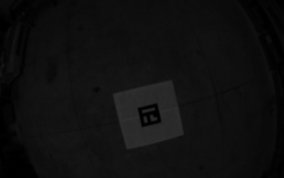
\includegraphics[width=\textwidth]{images/ling_apriltags_1.png}
	\end{subfigure}
	\begin{subfigure}[b]{0.45\linewidth}
		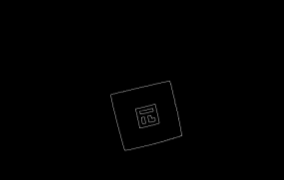
\includegraphics[width=\textwidth]{images/ling_apriltags_2.png}
	\end{subfigure}
	\caption{Ling's approach to optimizing AprilTags detection \cite{Ling2014}}
	\label{fig:ling_apriltags}
	\vspace{-0.4cm}
\end{figure}

In this work, the slow rate of state estimation was addressed using two novel ideas. First, the image size and calibration parameters are set depending on the distance between the quadrotor's position relative to the AprilTag. Secondly, we introduce the use of a Region of Interest (ROI) window to focus only on the AprilTag to reduce computational time required to estimate the pose. These novel ideas will be discussed in the following subsections.

\subsubsection{Adaptive Image Preprocessing}

As discussed previously, the low rate of the AprilTag library when processing images of 640 by 480 pixels results in an update rate of approximately 3 to 5 fps on a Snapdragon 8 core processor, which is too low to be used effectively in a PID control loop. Building upon the work of \cite{Ling2014}, who improved the AprilTag estimation rate by reducing the brightness on the image such that the majority of the pixels are black, additionally a set of image preprocessing methods such as Canny-Edge thresholding were also used. 

\subsubsection{Adaptive Image Windowing}

If one assumes that the quadrotor does not move to fast, there is relativity low rotation between image captures, and that the image update rate is quite fast (60 fps in this implementation), then the location the AprilTag in the following image can be estimated based off of the location it was last observed in the previous image. Therefore whenever an AprilTag is measured in an image, a bounding box around the AprilTag is calculated and then used in the following image to segment out portions of the image where the AprilTag is unlikely to be. An example of this implementation is highlighted in Figure \ref{fig:apriltags_windowing}. In cases where the AprilTag is not observed in the expected location (bounding box), the size of the bounding box is set to the size of the image and the entire image is processed. 

\begin{figure}[H]
	\centering
	\begin{subfigure}[b]{0.45\linewidth}
		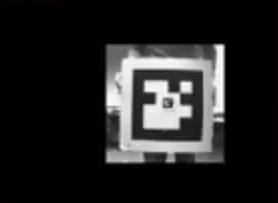
\includegraphics[width=\textwidth]{images/apriltags_roi_1.png}
	\end{subfigure}
	\begin{subfigure}[b]{0.45\linewidth}
		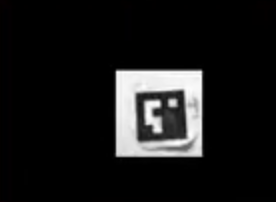
\includegraphics[width=\textwidth]{images/apriltags_roi_2.png}
	\end{subfigure}
	\caption{Adaptive Image Windowing}
	\label{fig:apriltags_windowing}
\end{figure}

While the adaptive windowing procedure decreases the computational resources needed for extracting pose estimates, there are two other problems that windowing cannot solve. First, as the size of the observed Apriltag increases, windowing is no longer adequate in decreasing computational time, this is an issue in cases where a high update rate is required (e.g. quadrotor landing). Second, in our use case as the observed AprilTag gets larger it becomes easy for the camera to lose track of the AprilTag itself, increasing the risk of no estimation for that time.

\subsubsection{AprilTag Inception}
To address both the decreasing state update rate as a function of proximity and reduce the probablity of losing sight of the AprilTag during landing a secondary AprilTag is embedded in the larger AprilTag, we term this technique AprilTag Inception (patent pending). This secondary AprilTag is assigned with a different family id to avoid confusion during detection, and is placed at the center of the larger primary AprilTag. Whenever the secondary AprilTag is captured in the image, the adaptive windowing method is set to track only the secondary AprilTag rather than the larger one, which reduces the portion of the image that must be processed in with each image capture. An example of this procedure is highlighted in Figure \ref{fig:apriltagInception}.
 
\begin{figure}[H]
	\centering
	\begin{subfigure}[b]{0.45\linewidth}
		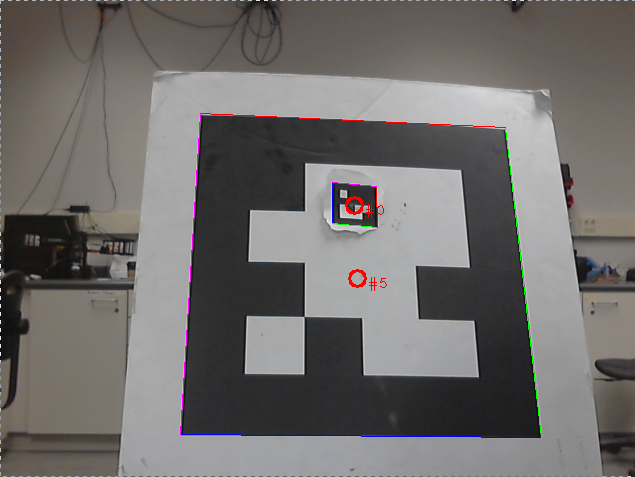
\includegraphics[width=\textwidth]{images/apriltags_1.png}
		\caption{2 Apriltags Detected}
	\end{subfigure}
	\begin{subfigure}[b]{0.45\linewidth}
		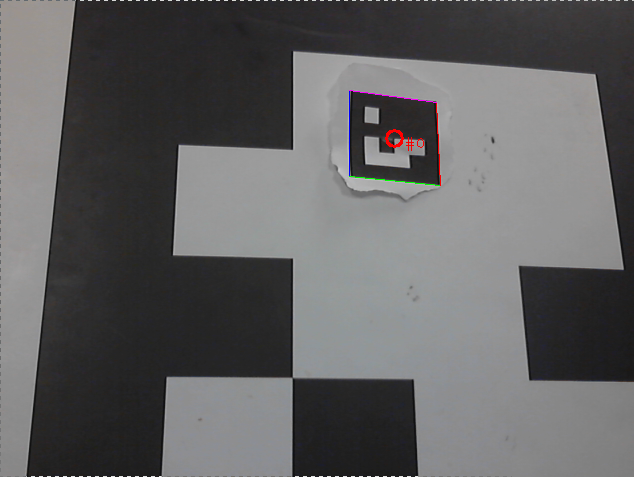
\includegraphics[width=\textwidth]{images/apriltags_3.png}
		\caption{1 Apriltag Detected }
	\end{subfigure}
	\caption{Apriltag Inception }
	\label{fig:apriltagInception}
\end{figure}

\subsubsection{Adaptive Image Down-sampling}
A final technique used to optimize the AprilTag detection was the introduction of down sampling the image size as the estimated distance between camera and AprilTag decreases. We devised 2 image down sampling sizes $320 \times 280$ (half resolution) and $160 \times 140$ (quarter resolution), when the distance between the camera and the AprilTag is less than 1.5 and 3 meters, the images are down sampled to the two resolutions respectively. If the camera is further than 3 meters from the AprilTag, the native resolution of $640 \times 480$ is used. This change only affected the image processing time when the quadrotor is within 3 meters of the quad and has the desired effect of maintaining a high AprilTag estimation rate.

In order to use down sampling effectively without corrupting the AprilTag estimations, 3 camera calibration files were also computed at the full, half and quarter camera resolutions, corresponding calibration files were then used with the AprilTag library during the state estimation procedure based on the current image resolution to obtain the correct pose estimates. 

\subsection{Controller and State Monitoring}
In this project we assumed that the quadrotor has successfully rendezvoused with the target vehicle and has a clear view through the camera image of the landing target located on the target vehicle at all times. The first step towards autonomous landing is to position the quadrotor above the landing target such that the displacements in the x and y directions in the horizontal plane normal to the landing surface are near zero while simultaneously matching speed and aligning the axis with the target vehicle. Next, while maintaining the near zero displacements in the x and y directions, the quadrotor descends at a safe rate such that the vertical distance between the quadrotor and the landing target is reduced until landing is achieved. Ideally the quadrotor will descend rapidly when the vertical displacement between the qaudrotor and target is large, slowing down just abvove ($\approx 1m$) the landing target inorder to minimize time and energy requirements of the landing maneouver. 

To achieve the described behaviour, we developed a PID position controller that outputs attitude commands such as roll and pitch to reduce the horizontal and vertical distance between the quadrotor and the landing platform, as well as an altitude command to maintain a safe approach altitude such that the target does not go out of view during landing. We omit yaw control as we assume the quadrotor will be axis aligned with the direction of travel of the moving target. 

The position controller takes the quadrotor's desired position and current position in $x$, $y$ and $z$ of the world frame as inputs, these inputs are mapped to attitude and altitude commands in the roll $\hat{\phi_t}$, pitch $\hat{\theta_t}$ and thrust $\hat{T_z}$ relative to the quadrotor frame as outlined in Equations \ref{eq:pid_roll}, \ref{eq:pid_pitch}, \ref{eq:pid_thrust}, these equations however assume that yaw $\psi$ is 0, if yaw is non-zero then roll and pitch need to be adjusted to account for the yaw changes as in Equation \ref{eq:pid_roll_adjusted} and \ref{eq:pid_pitch_adjusted}. The altitude command is adjusted when roll $\hat{\phi}$ and pitch $\hat{\theta}$ are non-zero to maintain altitude as in Equation \ref{eq:pid_thrust_adjusted}. 

\begin{equation}
	\label{eq:pid_error}
	e = e_{\text{setpoint}} - e_{\text{actual}}
\end{equation}

\begin{equation}
	\label{eq:pid_roll}
	\hat{\phi_t} = K_p e_x + K_i \sum_{t = 0}^{t} e_{x, t} dt + K_d \dot{e}_{x,t}
\end{equation}

\begin{equation}
	\label{eq:pid_pitch}
	\hat{\theta_t} = K_p e_y + K_i \sum_{t = 0}^{t} \dot{e}_{y,t} dt + K_d \dot{e}_{y ,t}
\end{equation}

\begin{equation}
	\label{eq:pid_thrust}
	\hat{T_z} =
		K_p e_z + K_i \sum_{t=0}^{t} \dot{e_z}_{,t} dt + K_d \dot{e_z}_{,t} 
\end{equation}

\begin{equation}
	\label{eq:pid_roll_adjusted}
	\phi_t = \cos(\psi_t) \hat{\phi_t} - \sin(\psi_t) \hat{\theta_t}
\end{equation}

\begin{equation}
	\label{eq:pid_pitch_adjusted}
	\theta_t = \sin(\psi_t) \hat{\phi_t} + \cos(\psi_t) \hat{\theta_t}
\end{equation}

\begin{equation}
	\label{eq:pid_thrust_adjusted}
	T = 
		T_{\text{hover}} +
		\frac{\hat{T_{z}}}{cos(\phi_t) cos(\theta_t)}
\end{equation}

\section{Experimental Hardware}
The quadrotor used in this experiment assembled from a DJI F450 quadrotor frame, 4 Emax 2213-935KV motors with complementary DJI E310 420S 20A electronic speed controllers. The flight controller selected for the project was a Pixhawk v2.4 running the PX4 firmware stack. An Odroid XU4 was selected as the onboard computer to processes captured images from a video stream and sends attitude commands via usb to the Pixhawk based of the PID controllers and current state as outlined above. Communication between the Odroid and the Pixhawk is handled by the mavros package which is a wrapper around the popular Mavlink communication protocal for UAVs.  Video was captured using a PointGrey Firefly 2.0 camera operating 60 frames per second (fps) with a resolution of 640 by 480 pixels along with a FujiFilm 135 degree FOV lens. The quadrotor and camera are highlighted in Figure \ref{Quadrotor}

\begin{figure}[H]
	\centering
	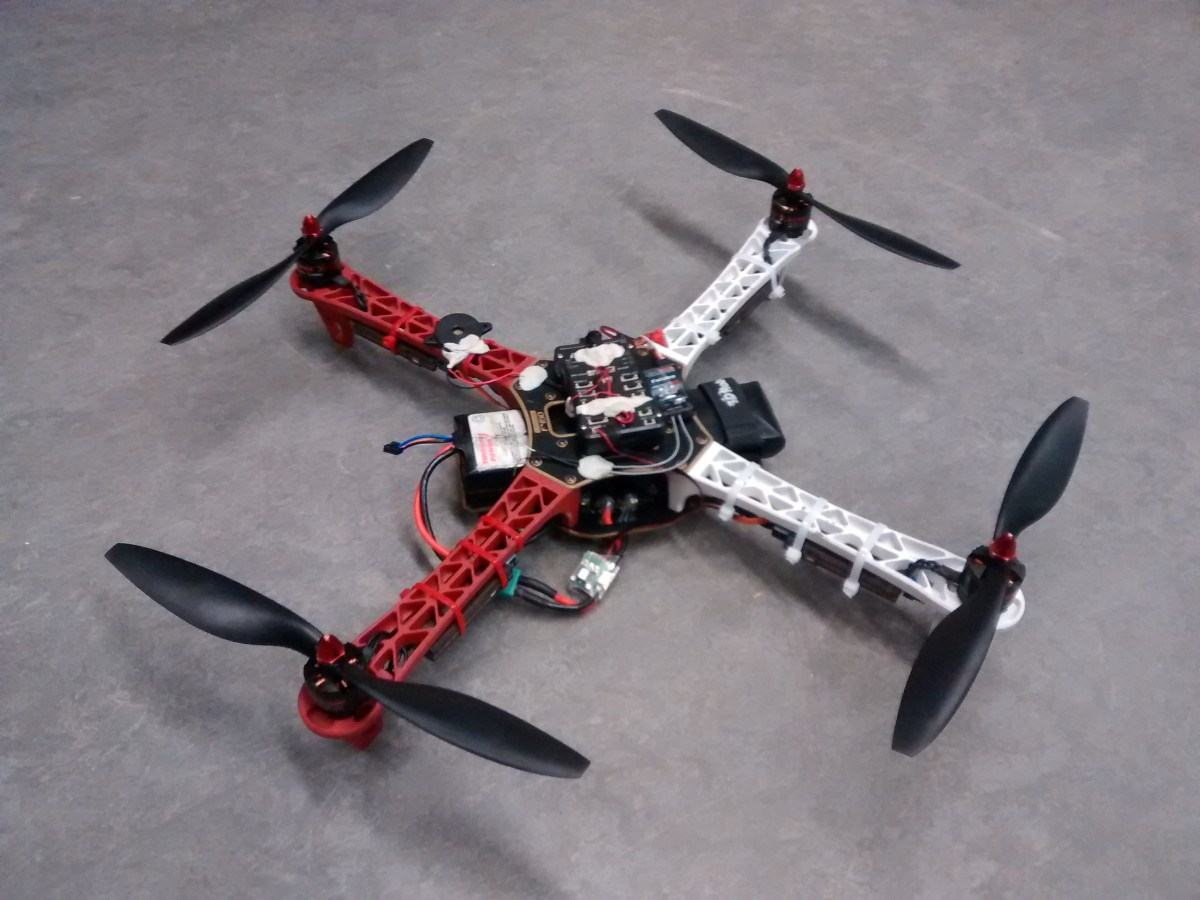
\includegraphics[width=0.8\linewidth]{images/quadrotor.jpg}
	\caption{DJI F450 with Pixhawk v2.4}
	\label{Quadrotor}
\end{figure}


\section{Results}
\begin{itemize}
	\item Results of the image stuff
	\begin{itemize}
		\item Plot of FPS vs distance
		\item Plot of true state vs mocap state?
	\end{itemize}
	
	\item PID/Control results 
	\begin{itemize}
		\item Plot XY for the controller loop
		\item Optimal PID settings
		\item How we got there
		\item Decent plot (V as a function of Z)
		\item Video?
	\end{itemize}
	
\end{itemize}

\subsection{AprilTag Results}
\begin{figure}
	\centering
	\begin{subfigure}[b]{\linewidth}
		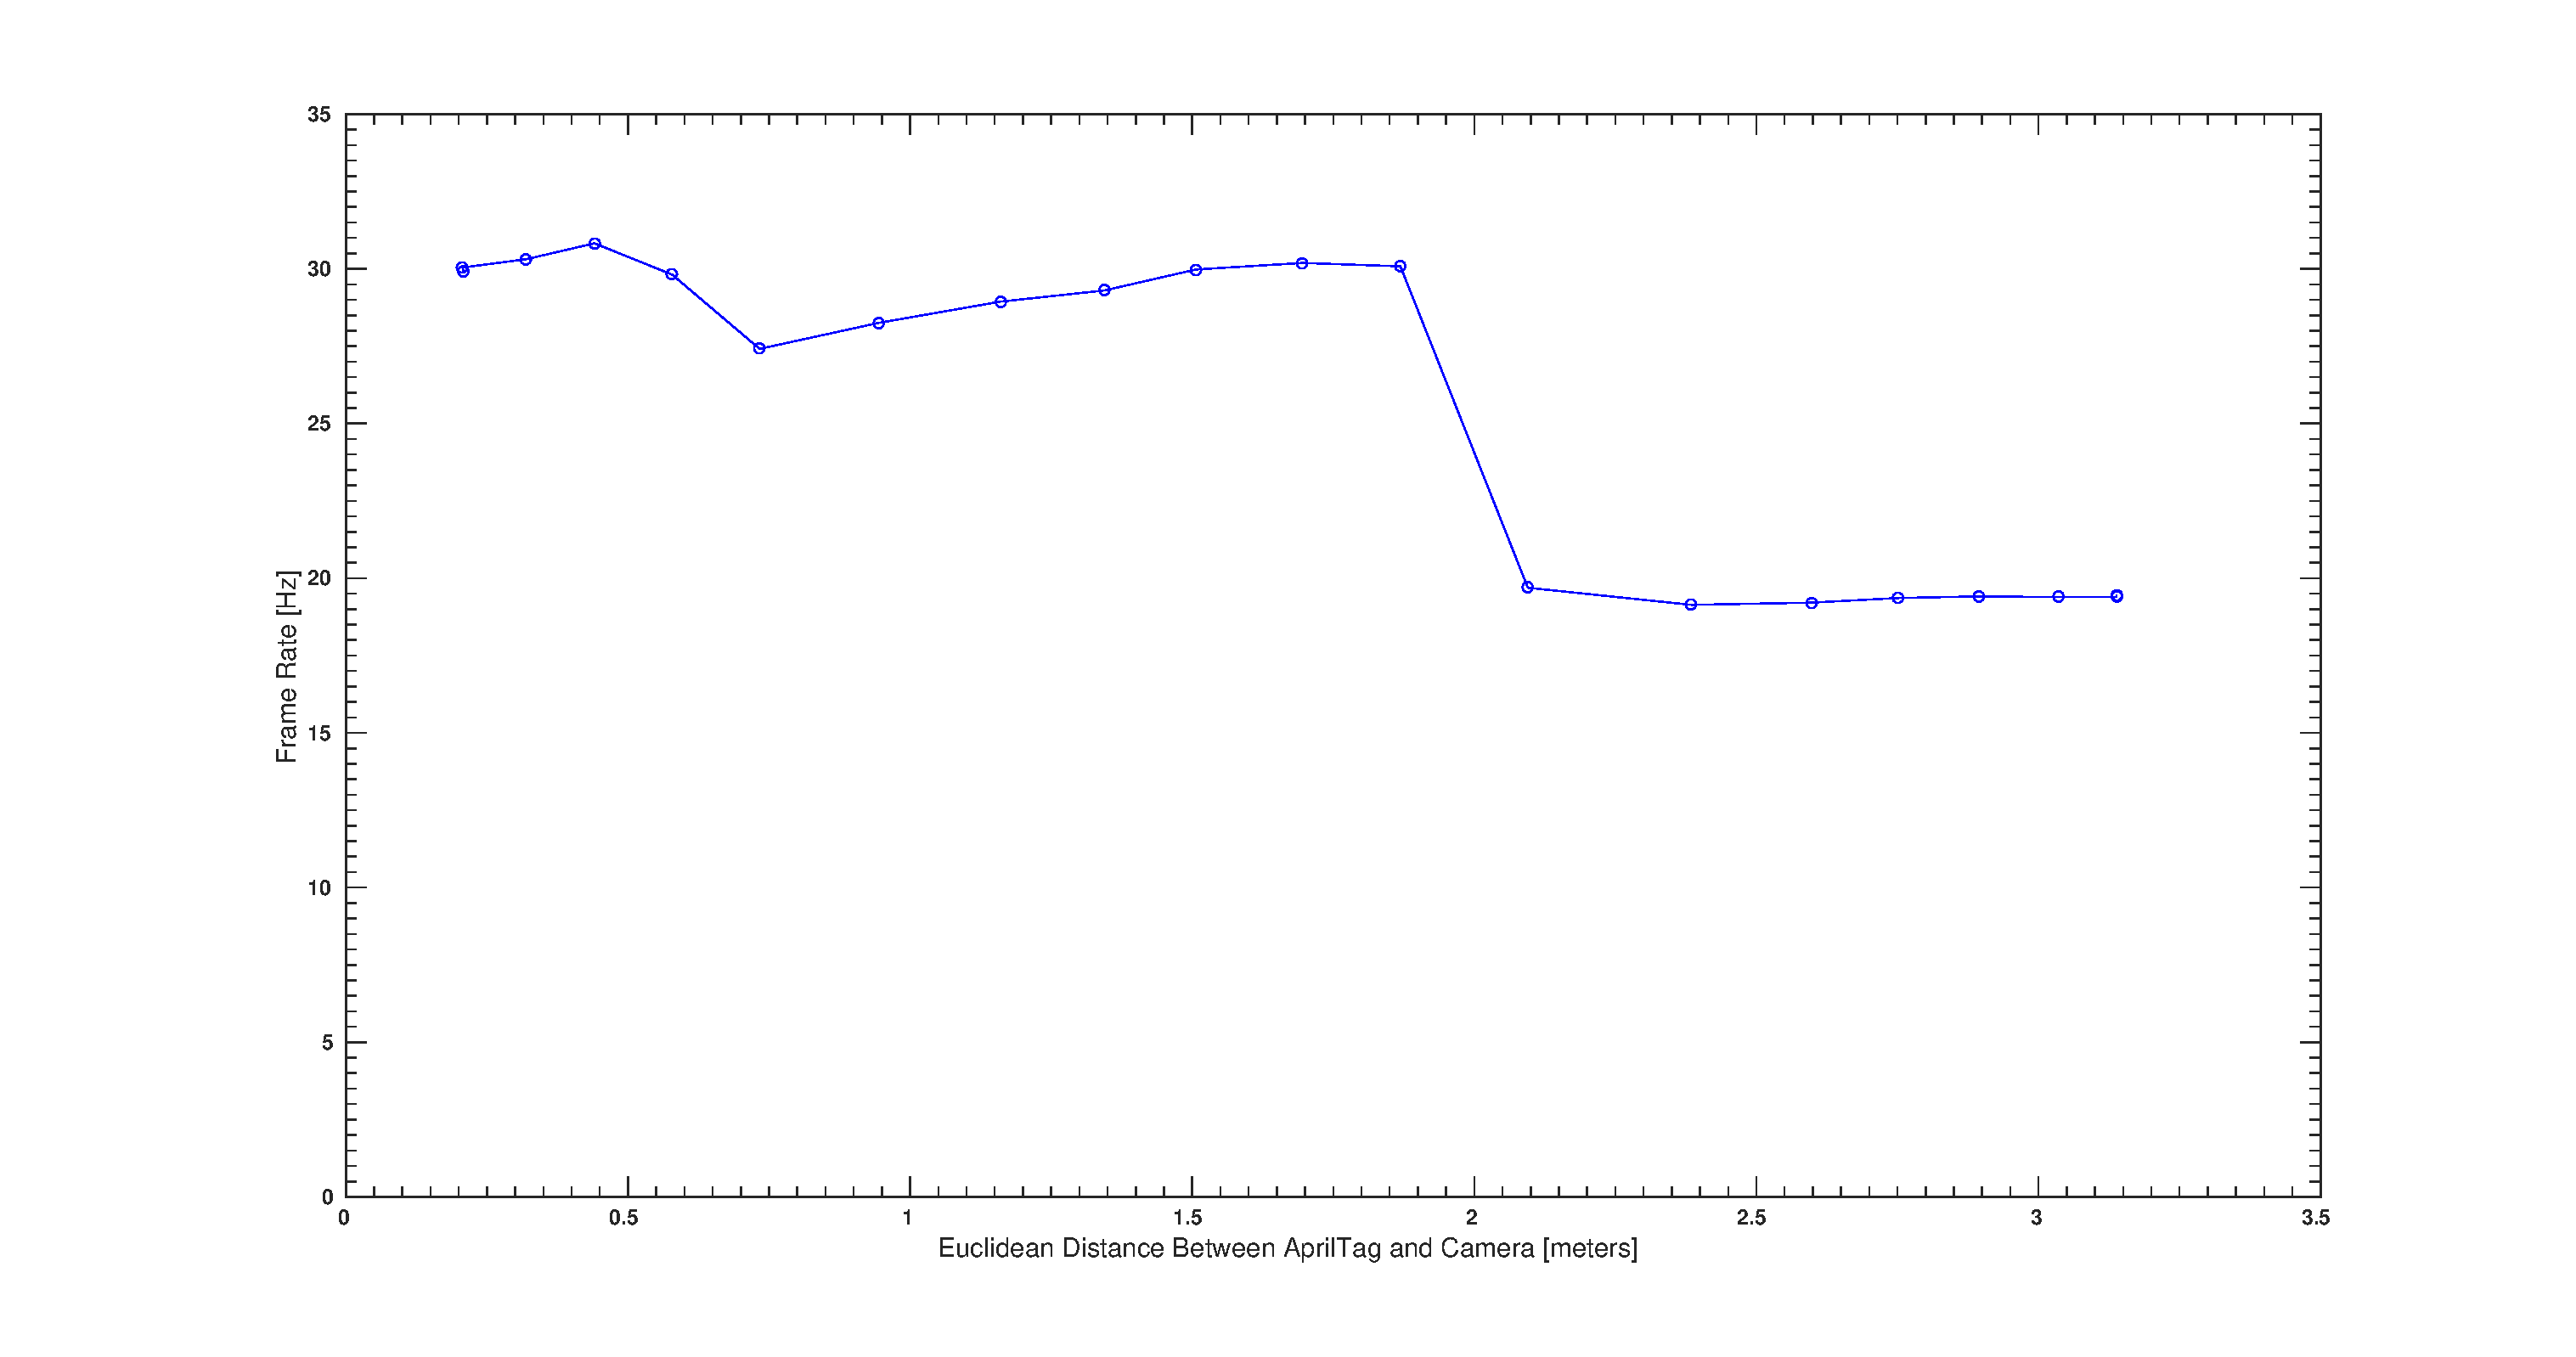
\includegraphics[width=\textwidth]{images/Apr_FPS_vs_Dist.eps}
		\caption{}
		\label{fig:pid_roll}
	\end{subfigure}

	\begin{subfigure}[b]{\linewidth}
		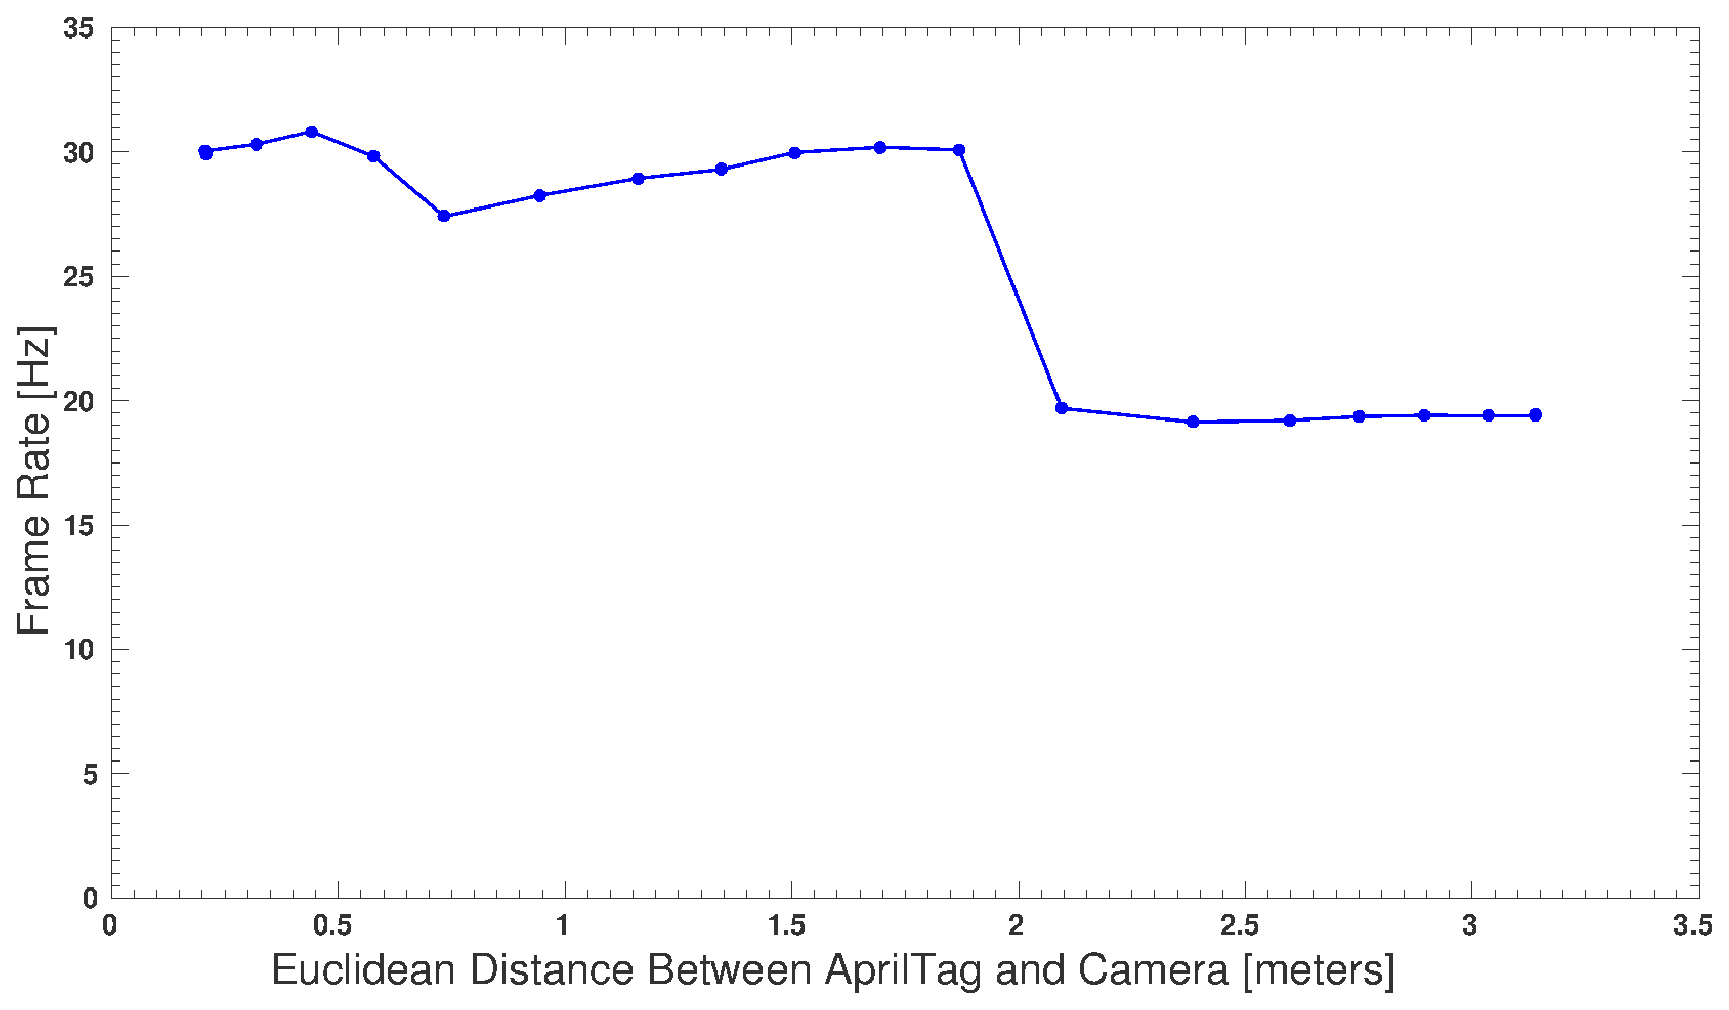
\includegraphics[width=\textwidth]{images/Apr_Distance_Error.eps}
		\caption{}
		\label{fig:pid_roll}
	\end{subfigure}
\end{figure}



\subsection{PID and Controller Results}

\begin{figure*}
	\centering
	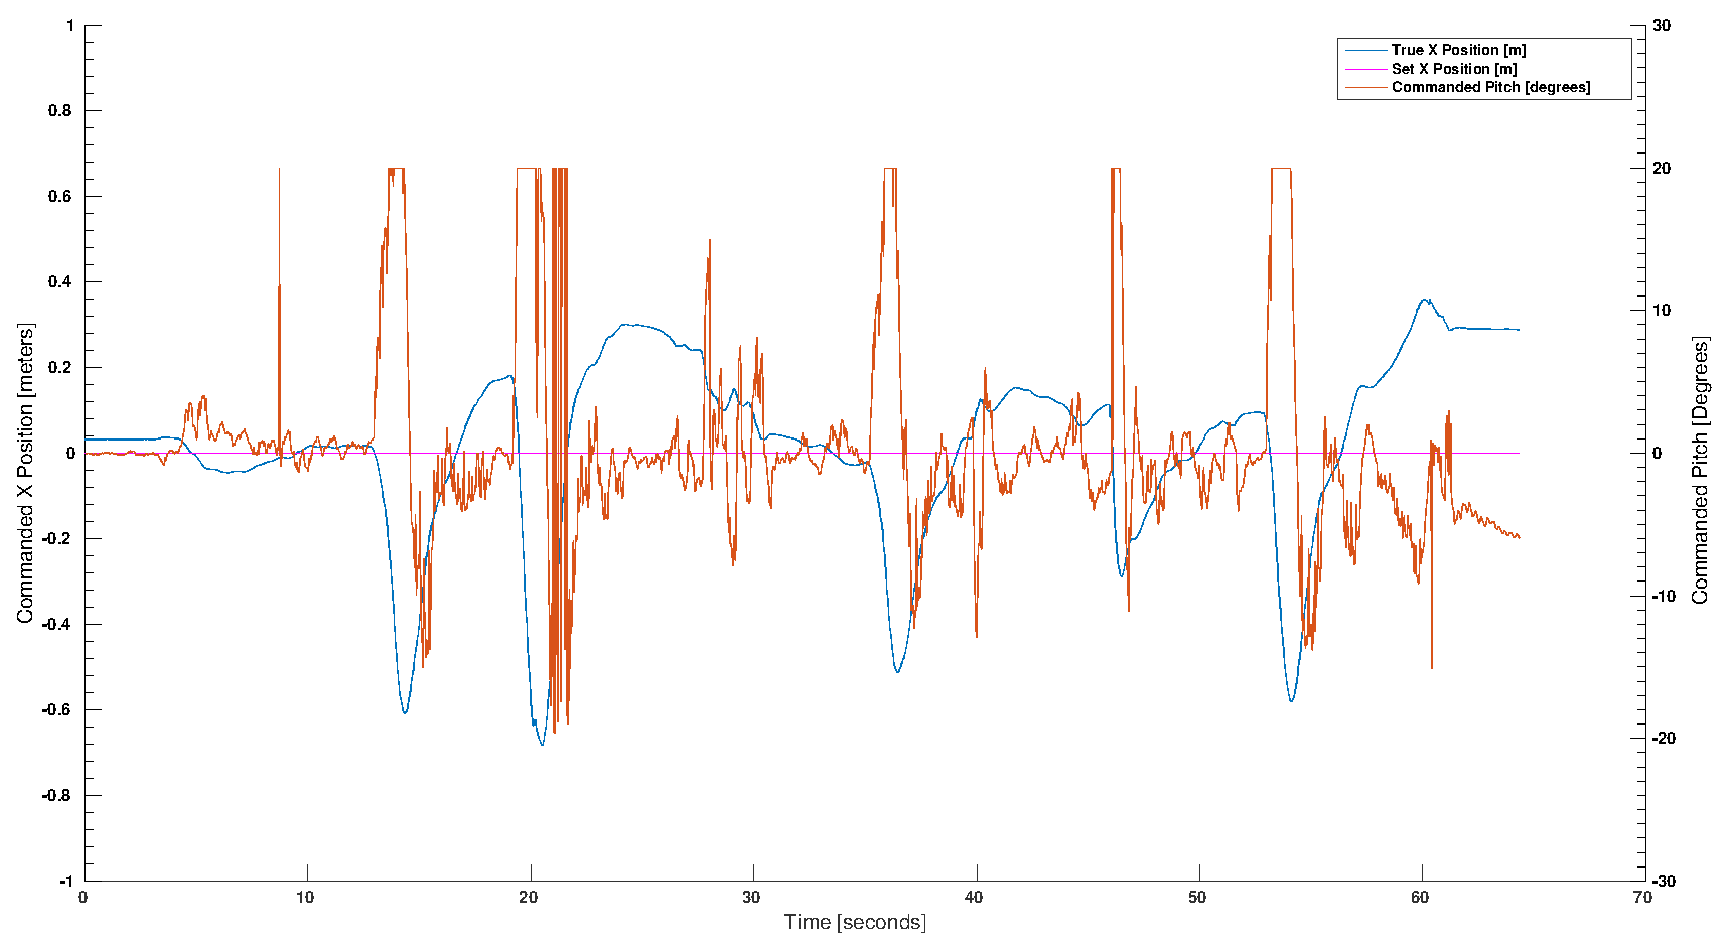
\includegraphics[width=\textwidth]{images/PID_Pitch_x_true_and_obs.eps}
	\caption{Position Controller - Pitch Command}
	\label{fig:pid_roll}
\end{figure*}

\begin{figure*}
	\centering
	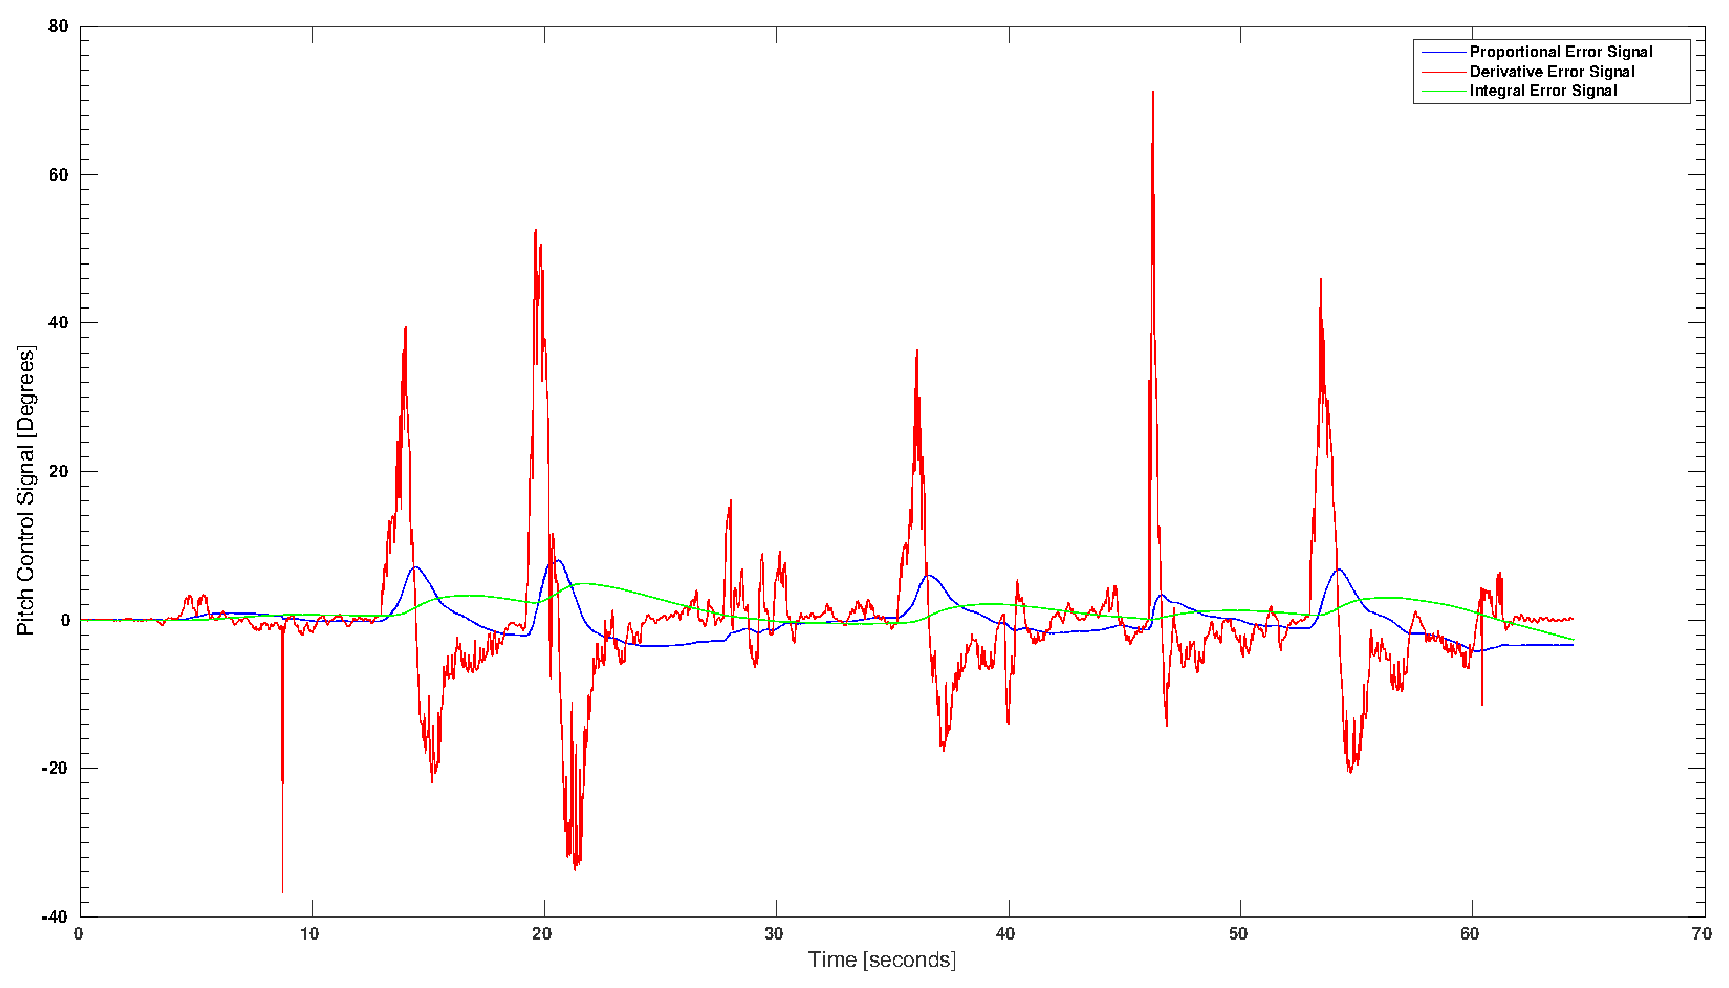
\includegraphics[width=\textwidth]{images/PID_Pitch_Controls.eps}
	\caption{Position Controller - Pitch Control Signal Components}
	\label{fig:pid_roll}
\end{figure*}

\begin{figure*}
	\centering
	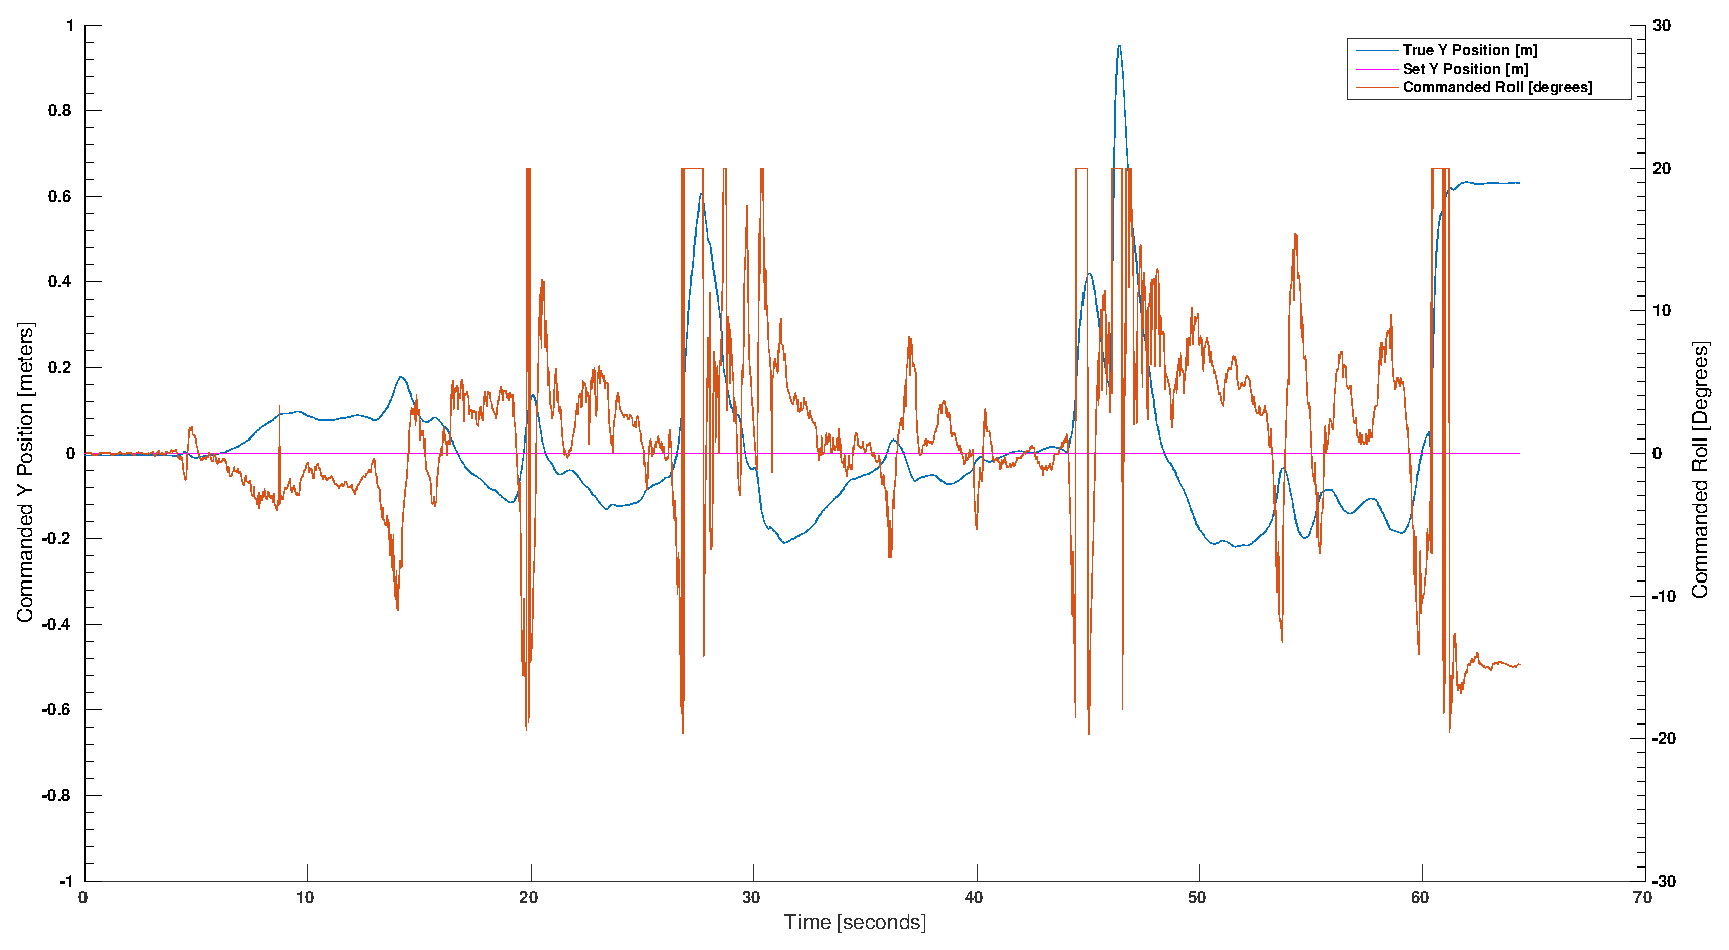
\includegraphics[width=\textwidth]{images/PID_Roll_y_true_and_obs.eps}
	\caption{Position Controller - Roll Command}
	\label{fig:pid_roll}
\end{figure*}

\begin{figure*}
	\centering
	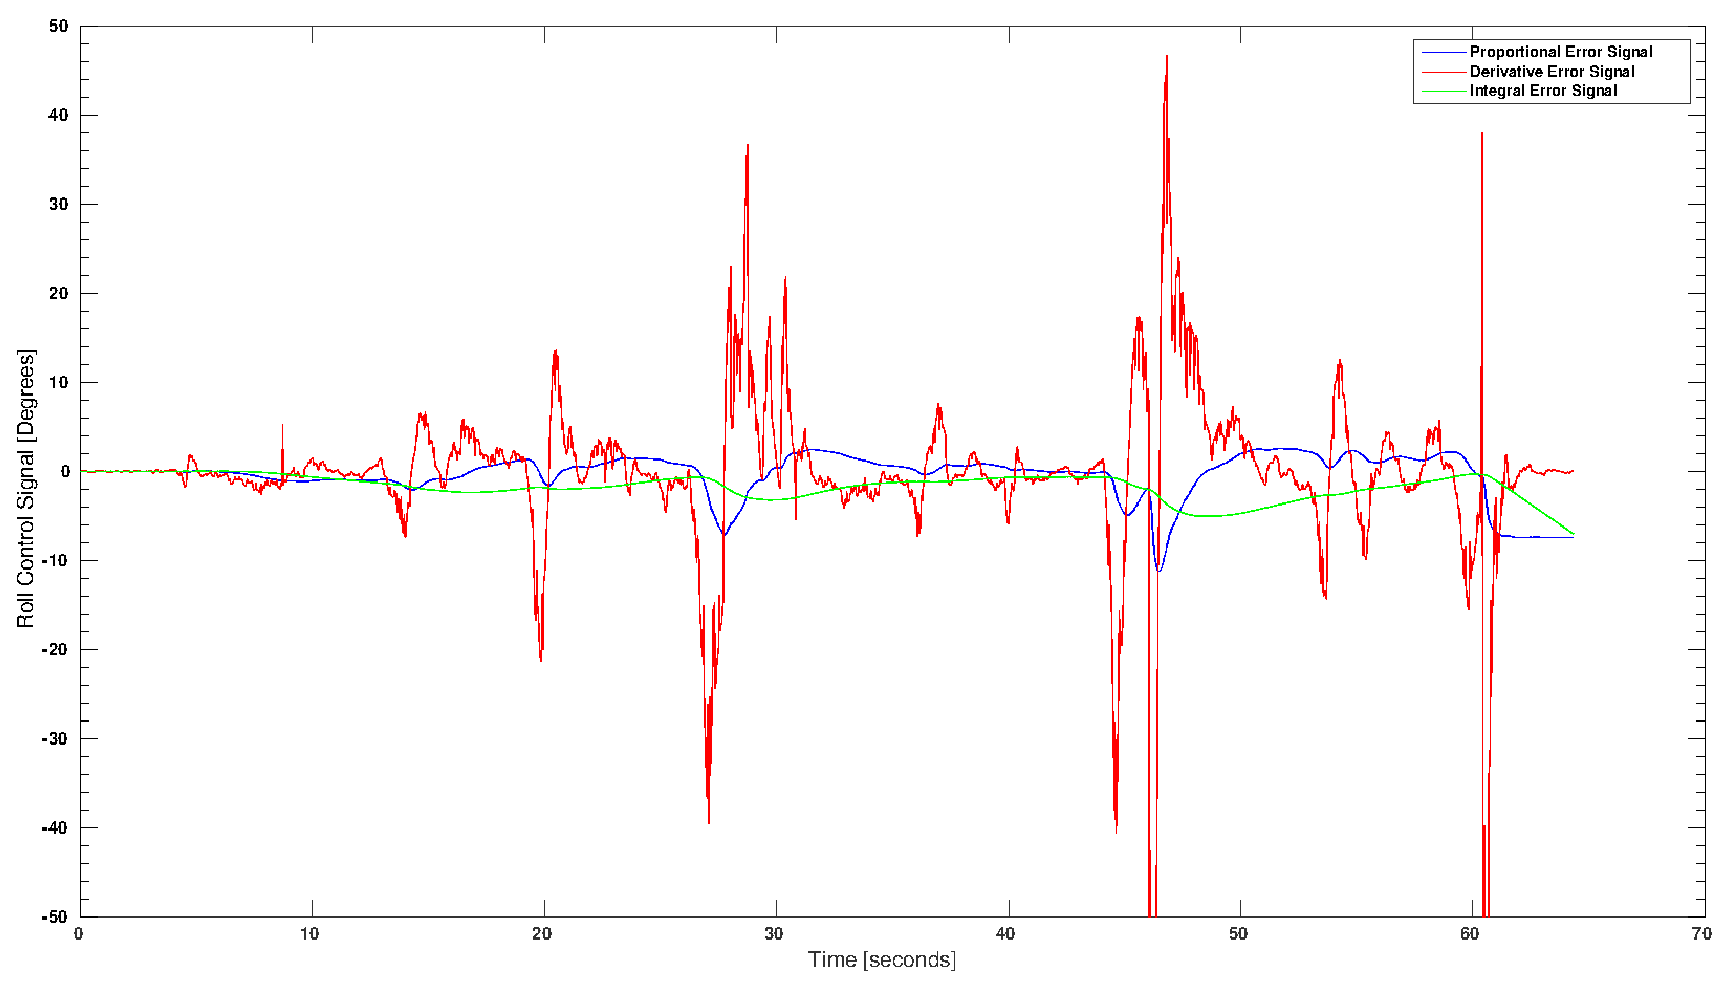
\includegraphics[width=\textwidth]{images/PID_Roll_Controls.eps}
	\caption{Position Controller - Roll Control Signal Components}
	\label{fig:pid_roll}
\end{figure*}

\begin{figure*}
	\centering
	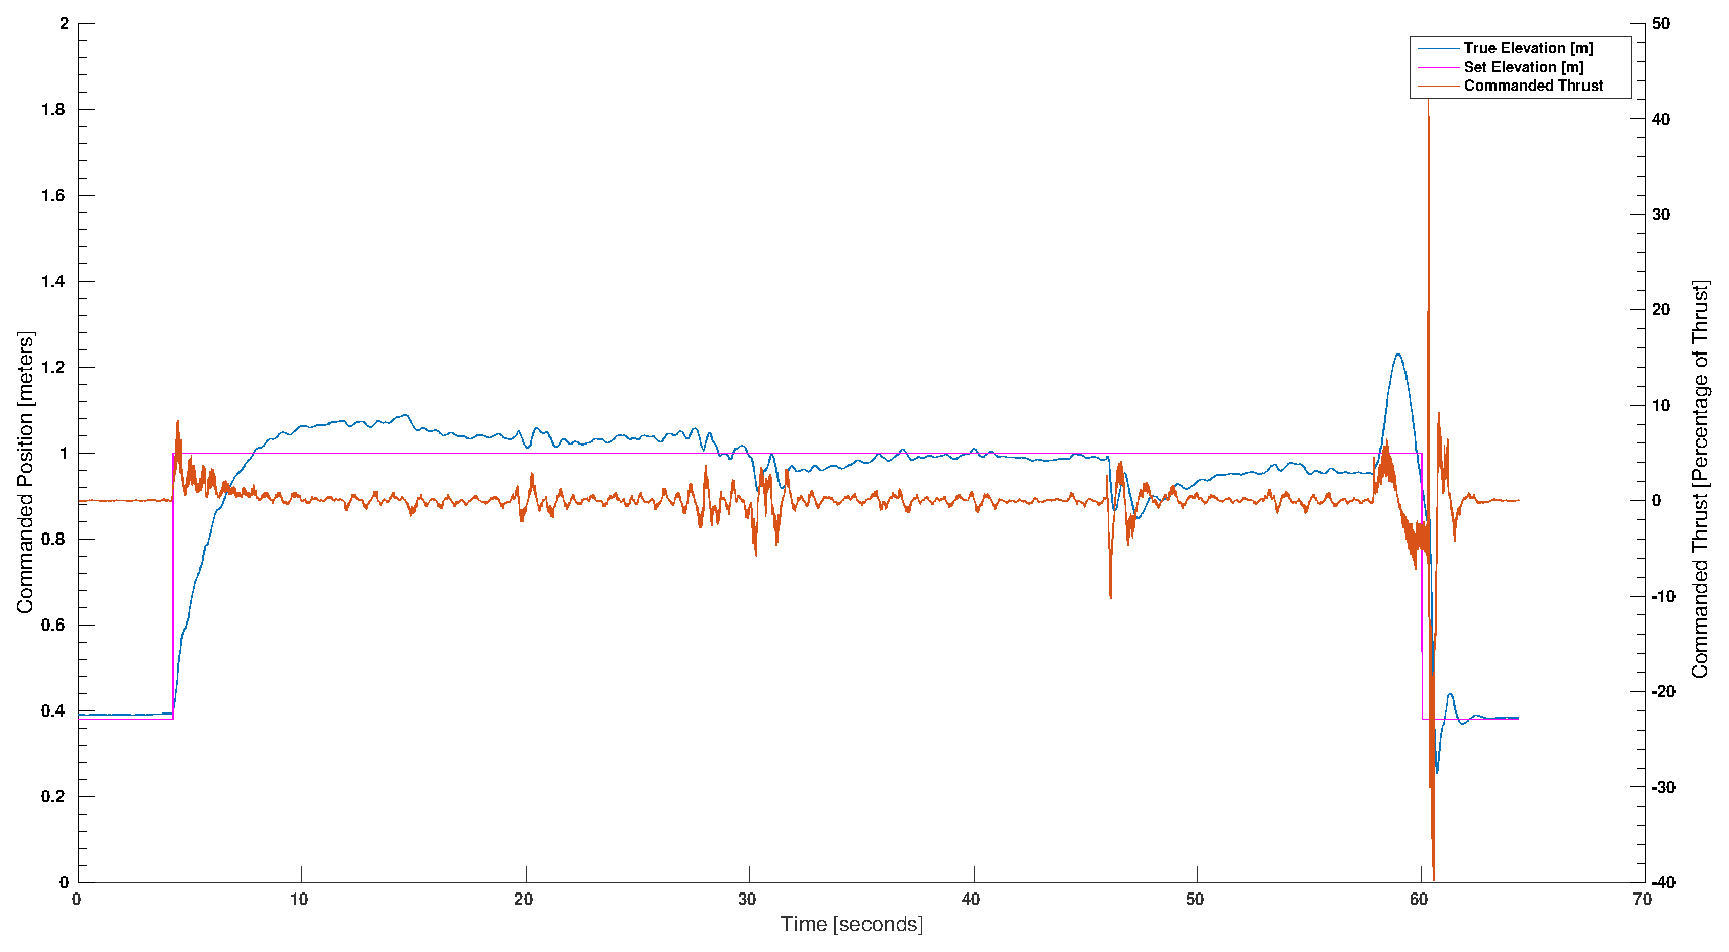
\includegraphics[width=\textwidth]{images/PID_Elevation_True_and_obs.eps}
	\caption{Position Controller - Thrust Command}
	\label{fig:pid_roll}
\end{figure*}

\begin{figure*}
	\centering
	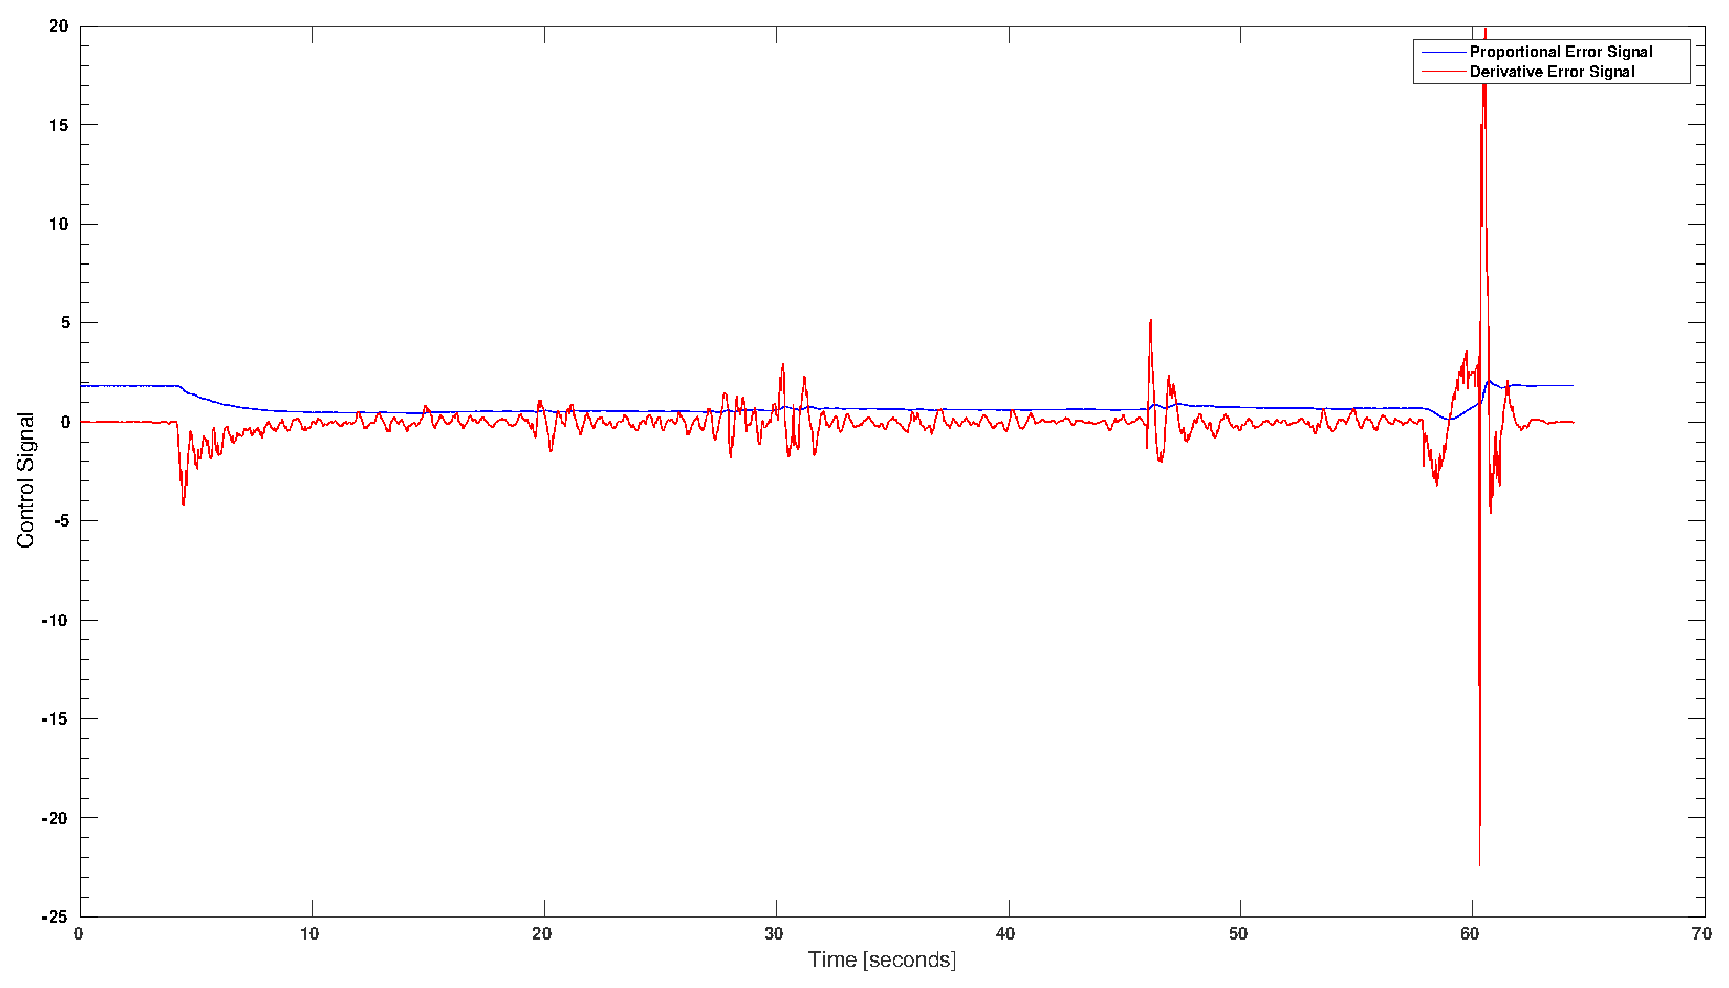
\includegraphics[width=\textwidth]{images/PID_Elevation_Controls.eps}
	\caption{Position Controller - Thrust Signal Components}
	\label{fig:pid_roll}
\end{figure*}

So far the PID behaviours and gains have only been evaluated using a MOCAP system and tested only relative to a stationary target and these results are discussed herein. 




\section{Conclusion and Future Work}


\section{Proposed Future Work}
In the coming weeks, the PID controllers tested and developed using the MOCAP system will be tested using state estimates that are produced from the AprilTag library and the image preprocessing methods outlined in section \textbf{\textit{OUTLINE OF IMAGE PREPROCESSSING}}. 

One major issue highlighted in Ling \cite{Ling2014} is that due to the relatively long processing time of the AprilTags library, the estimated state obtained at a time $t$ does not actually represent the current state due to a time lag. This time lag as outlined in \cite{Ling2014} and defined in \ref{Detection Delay} must be accounted for when using the camera to estimate state. Currently our proposed method to measure this lag is to use the MOCAP system to provide a ground truth for the state from which we can estimate the estimated state.  

\begin{equation}
\label{Detection Delay}
    t_{\text{capture}} = t - \delta t_{\text{camera}} + \delta t_{\text{detection}}
\end{equation}

The next issue that will need to be address is the problem of the camera view. The dynamics of a quadrotor work in such a way that in order to move towards a goal point, the quadrotor must tilt away from the target which leads to problems with maintaining a view of the target when desired roll or pitch angles are greater than approximately 10 degress. This issue can either be addressed by mounting the camera at an angle or by adding a gimbals to the the quadrotor such that the gimbal will be sent commands by the onboard computer that will maintain a constant view of the target regardless of the commanded roll and pitch. 

Both of the above solutions have significant implementation questions that will have to be answered. If using the fixed camera angle, then the yaw of the qaudrotor will need to be controlled by a PID controller, similar to the the PID controllers to the roll and pitch. In the case of significant wind, the quadrotor will need to rotate itself such that the front of the quad is pointed into the wind during the final decent.

If a gimbal is used there are two issues that arise. First a new set of controllers that send roll, pitch and yaw commands to the gimbal such that the camera it is attached to maintains a centred view of the target platform must be developed. These controllers will likely be similar to the PID controllers developed above and so they are not considered to be terrible difficult to define are implement. The more difficult part of using a gimbal is related to resuming the gimbal state, which in cheaper gimbals do provide. All of the gimbals that have been researched as part of this project do not provide state feedback and so they are considered to be open loop. Therefore in order to use such a gimbal the user will need to assume the commanded gimbal position is equal to the true gimbal position, from which a transform between the quad rotor and the gimbal can be made.








\bibliography{report}{}
\bibliographystyle{ieeetr}






\end{document}
